\documentclass{classrep}
\usepackage[utf8]{inputenc}
\frenchspacing

\usepackage{graphicx}
\usepackage[usenames,dvipsnames]{color}
\usepackage[hidelinks]{hyperref}
\usepackage{lmodern}
\usepackage{placeins}
\usepackage{amsmath, amssymb, mathtools}
\usepackage{listings}
\usepackage{fancyhdr, lastpage}

\pagestyle{fancyplain}
\fancyhf{}
\renewcommand{\headrulewidth}{0pt}
\cfoot{\thepage\ / \pageref*{LastPage}}

%--------------------------------------------------------------------------------------%
\studycycle{Informatyka stosowana, studia dzienne, II st.}
\coursesemester{I}

\coursename{Wprowadzenie do Data Science i metod uczenia maszynowego}
\courseyear{2020/2021}

\courseteacher{mgr inż. Rafał Woźniak}
\coursegroup{Wtorek, 13:15}

\author{%
    \studentinfo[239676@edu.p.lodz.pl]{Kamil Kowalewski}{239676}
}

\title{Zadanie 1.: Problem Set 1}

\begin{document}
    \maketitle
    \thispagestyle{fancyplain}

    \section{Wprowadzenie}
    \label{intro} {
        Bardzo częstym zjawiskiem jest manipulacja danymi tak, aby zmylić odbiorcę
        i~zmusić go, aby myślał, tak ja chciał autor danego tekstu czy też przekazu.
        Może być to realizowane w zróżnicowany sposób natomiast poniżej zostanie
        omówiony problem o nazwie \emph{Korelacja a przyczynowość}
        (ang. \emph{Correlation vs Causation}). Polega on na powiązaniu dwóch tematyk
        czy też zjawisk, jakie mają miejsce i są brane pod uwagę w danych badaniach.
        Można hipotetycznie założyć, że mamy dwie zmienne \textit{X} oraz \textit{Y}
        i~wystepuję między nimi korelacja, czyli zależność jednej od drugiej. Zależność
        ta wyraża się w ten sposób, że przykładowo gdy dwie zmienne \textit{X}
        oraz \textit{Y} wzrastają razem, oraz maleją razem. Celem wyjaśnienia tego można
        wyróżnić parę scenariuszy, pierwsze z nich jest to, że zjawisko określone jako
        zmienna \textit{X} powoduje zjawisko określone przez zmienną \textit{Y}.
        Kolejnym przypadkiem jest to, że zjawisko określone przez zmienną \textit{Y}
        może powodować zjawisko określone przez zmienną \textit{X}. Trzecią opcją jest
        to, że istnieję dodatkowa, trzecia zmienna, która wpływa na wcześniej już
        wspomniane zmienne \textit{X} oraz \textit{Y}. Ostatnią z możliwości jest to,
        że zmienne \textit{X} oraz \textit{Y} są totalnie z sobą niezwiązane a autor
        artykułu powiązał je, aby osiągnąć swój cel i zmanipulować przesłaniem a co za
        tym idzie wnioskami, jaki wyciągnie z nich czytelnik.
    }

    \section{Przykłady błędnie dobranych zjawisk}
    \label{wrong_examples} {

        \subsection{Wykorzystanie stereotypów i obiegowych opinii}
        \label{wrong_examples:stereotypes} {
            Jednym z ciekawych przykładów obrazujących zjawisko manipulacji jest
            przedstawiony w artykule \cite{medium_article} sytuacja połączenia palenia
            papierosów przez uczniów oraz uzyskiwanych przez nich ocen. Autor próbuje
            narzucić czytelnikowi tezę, że to właśnie przez palenie papierosów uczniowie
            uzyskują gorsze wyniki w nauce, co jest mocno ugruntowane w społeczeństwie, że
            osoby, które mają styczność ze środowiskami patologicznym zazwyczaj posiadają
            niskie wykształcenie. Autor wykorzystuję tutaj częstą opinię czy też
            stereotyp. Warto się odnieść tutaj do sekcji \ref{intro} gdzie zostało
            opisane, że zależność może działać w drugą stronę, że właśnie to te złe
            oceny czy też niepowodzenia w nauce powodują chęć skorzystania ze wcześniej
            wspomnianej używki celem rozładowania stresu czy też doznania przyjemność z
            jej przyjmowania. Patrząc na sprawę w wyższego pułapu można też dojść do
            wniosku, że po prostu osoby z patologicznych rodzin mają skłonność do
            korzystania z używek w młodym wieku i nie zależy im na edukacji, gdyż
            po prostu mieli takie wzorce w domu. Jest to przypadek z tą trzecią zmienną
            przedstawiony w sekcji \ref{intro}.
        }

        \subsection{Korelacja zmiennych bez związku}
        \label{wrong_examples:no_relationship} {
            Drugim z przykładów błędnie dobranej korelacji jest zauważenie przez autora
            korelacji dwóch zmiennych natomiast brak refleksji, że nie są one ze sobą
            totalnie powiązane. Warto tutaj od razu wspomnieć, że korelacja nie
            implikuje przyczynowości. To niezmiernie dobrze, że autor zauważył taką
            pozytywną przemianę w przeciągu tych paru lat przedstawioną na rysunku
            \ref{margarine_divorces} natomiast powinno zostać to odrzucone jako
            bezsensowne porównanie.

            \begin{figure}[!htbp]
                \centering
                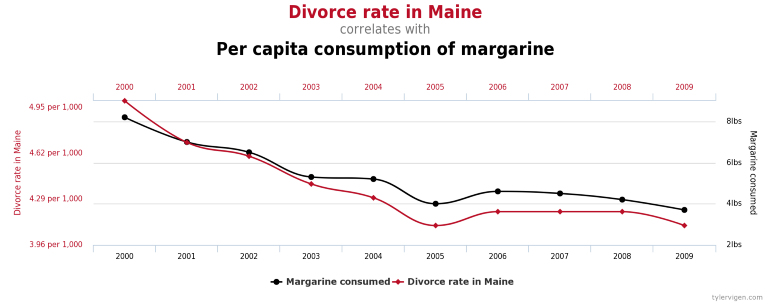
\includegraphics
                [width=\textwidth,keepaspectratio]
                {img/margarine_divorces.png}
                \caption
                [Wykres spożycia margaryny oraz liczby rozwodów w danych latach]
                {Wykres spożycia margaryny oraz liczby rozwodów w danych latach}
                \label{margarine_divorces}
            \end{figure}
            \FloatBarrier
        }

        \subsection{Korelacja tylko na danym przedziale liczbowym}
        \label{wrong_examples:interval} {
            Wartym uwagi jest również fakt, iż wykresy w danych artykułach obejmują
            pewien ograniczony przedział np. czasu. Zazwyczaj autor dobiera go sobie
            tak, aby wykazać, to co miał na celu. Niezwykle ważne jest to, że w danym
            przedziale dwie czy też więcej zmiennych mogą się zachowywać w sposób
            liniowy natomiast na szerszym przedziale jedna z nich może mieć przebieg
            logarytmiczny. W takiej sytuacji patrzeć na wykres korelacja może być
            bardzo słabo zauważalna a wręcz można wyjść z hipotezą, że ona nie występuję.
            Świetnym przykładem przedstawionym w artykule
            \cite{towardsdatascience_article} jest odczucia szczęścia życiowego w
            stosunku do zarobków rocznych. Przedstawiając tylko początkowy fragment
            tego wykresu czytelnik może dojść do wniosku, że im większy roczny zarobek
            tylko wyższy poziom szczęścia, czyli np. Bill Gates byłby w elitarnym gronie
            osób o najwyższym poziomie szczęścia na naszej planecie. Niestety tak nie
            jest, ponieważ powyżej pewnej określonej kwoty ilość pieniędzy przestaja
            podnosić poziom szczęścia a często nawet go obniża. Stąd jest tak ważna
            refleksja autora, aby podać dane, które rzetelnie oddają pewną zależność.
        }
    }

    \section{Rozwiązanie problemów}
    \label{good_examples}{
        Rozwiązanie problemów przedstawionych w sekcji \ref{wrong_examples} z pewnością
        nie są banalne natomiast poniżej autor tego tekstu chciałbym się
        odnieść i przedstawić zbiór sugestii, które jego zdaniem mogłyby wyeliminować
        lub chociaż zmniejszyć liczbę tych błędów.

        Odnosząc się do problemu w sekcji \ref{wrong_examples:stereotypes} autorzy
        tekstów powinni powstrzymać swoje ambicje i ego na rzecz przedstawiania
        rzetelnych danych i niewprowadzanie w błąd czytelników natomiast sami
        czytelnicy powinni posiadać wysoki poziom świadomości i podchodzić bardzo
        krytycznie do przedstawianych im informacji i w miarę możliwości samemu
        weryfikować informacje, jakie otrzymują, aby nie dać się zmanipulować.

        Odnosząc się do problemu w sekcji \ref{wrong_examples:no_relationship} autorzy
        powinni przed wykorzystaniem danej zależność bardzo dokładnie przemyśleć czy ma
        ona sens. Prawie każdy inteligentny i myślący odbiorcą z pewnością zauważy
        bezsensowność porównania, przez co odbiór przygotowane tworu intelektualnego może
        być negatywny a sama jego ocena może być niezwykle niska. Może to skutkować
        tym, że opinia o danym autorze będzie niska i z czasem zostanie on wyparty
        przez innych bardziej rzetelnych twórców.

        Odnosząc się do problemu w sekcji \ref{wrong_examples:interval} w szczególności
        odbiorcy powinni być szczególne uwrażliwieni na tę sytuację, gdyż mogą być łatwy
        sposób zmanipulowani. Po stronie autorów powinien istnieć pewien kodeks moralny
        rzetelnego przedstawiania danych. Gdy nawet nie mają możliwość pełnego
        przedstawienia powinni zasygnalizować o fakcie, że przedstawione dane mogą dawać
        mylny obraz sytuacji.
    }

    \section{Wnioski} {
        Podsumowując można powiedzieć, że:
        \begin{itemize}
            \item ...

        \end{itemize}
    }

    \begin{thebibliography}{0}
        \bibitem
        {medium_article}
        {https://medium.com/seek-blog/how-to-lie-with-statistics-b671b66399d}
        \bibitem
        {towardsdatascience_article}
        {https://towardsdatascience.com/lessons-from-how-to-lie-with-statistics-57060c0d2f19}
    \end{thebibliography}

\end{document}
